\documentclass[]{article}


\usepackage{tabularx}
\usepackage{booktabs}
\usepackage{grid-system}
\usepackage{graphicx}
\usepackage{subcaption}
\usepackage[margin=0in,paperheight=1550pt]{geometry}
\usepackage{amsmath}
\usepackage{moresize}
\usepackage{xcolor}
\usepackage{pagecolor}
\usepackage{hyperref}
\usepackage{fontawesome5}

\definecolor{background}{RGB}{216, 180, 118}
\definecolor{header}{RGB}{116, 180, 118}
\pagecolor{background}

% no word break https://tex.stackexchange.com/questions/5036/how-to-prevent-latex-from-hyphenating-the-entire-document/5039
\tolerance=1
\emergencystretch=\maxdimen
\hyphenpenalty=10000
\hbadness=10000

\newcommand{\lcol}{0.15}
\newcommand{\ccol}{0.55}
\newcommand{\rcol}{0.25}
\newcommand{\textsize}{\large}

\begin{document}
	\begin{figure}[b]
		\centering
		\begin{subfigure}{.2\linewidth}
		    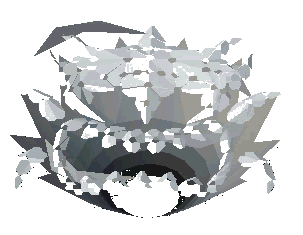
\includegraphics[width=1.5\linewidth]{../../docs/latex/img/general/skill_capes/transparent_Howling_Snow_Storm-0.png}
		\end{subfigure}%
		\begin{subfigure}{.6\linewidth}
			\centering
		    \Huge{\textbf{Optimizing Runescape}}
		    \vspace{5mm}
		    \huge{\textit{Wintertodt}}
		\end{subfigure}%
		\begin{subfigure}{.2\linewidth}
		    
\includegraphics[width=0.6\linewidth]{../../docs/latex/img/general/skill_capes/Firemaking_cape_detail.png}
		    \vspace{5mm}
		\end{subfigure}

		\hrule
		\centering
		\begin{subfigure}{\lcol\linewidth}
		    \centering
		    \LARGE{\textbf{Actions}}
		\end{subfigure}%
		\begin{subfigure}{\ccol\linewidth}
		    \centering
		    \vspace{5mm}
		    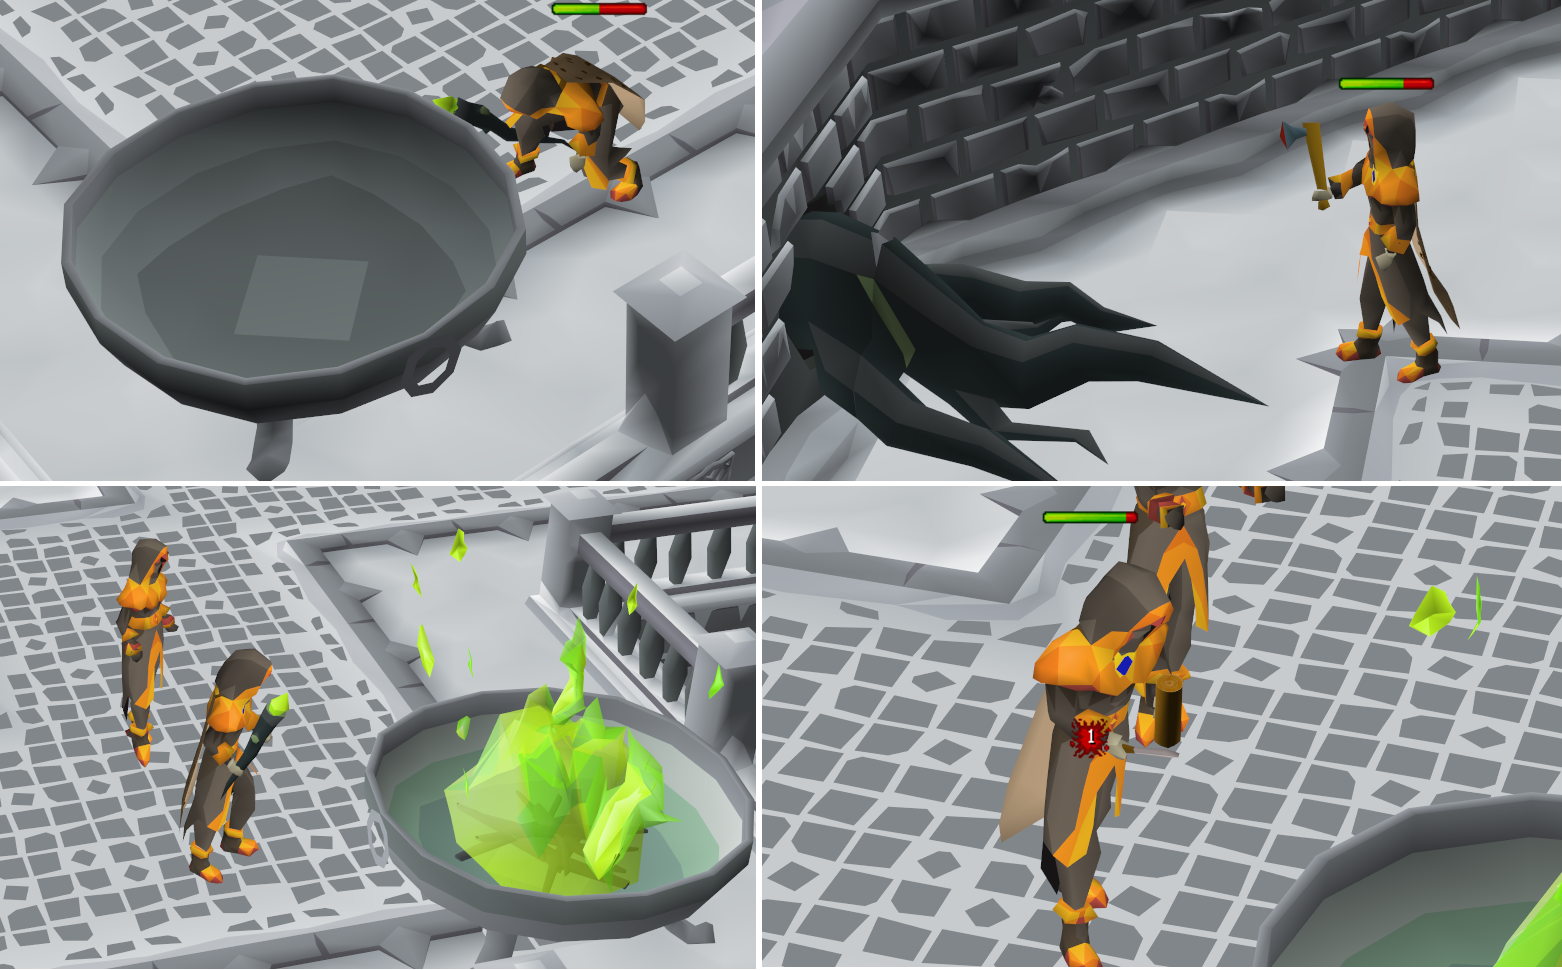
\includegraphics[width=0.9\linewidth]{../../docs/latex/img/firemaking/wintertodt_actions.png}
		    \vspace{5mm}
		\end{subfigure}%
		\begin{subfigure}{\rcol\linewidth}
			\textsize
		    A player can perform several actions during a game. Some of them give firemaking experience. We can model this skilling boss to gain insight, make predictions, and guide players.
		\end{subfigure}

		\hrule

		\begin{subfigure}{\lcol\linewidth}
		    \centering
		    \LARGE{\textbf{Policies}}
		\end{subfigure}%
		\textsize
		\begin{subfigure}{\ccol\linewidth}
		    \begin{gather*}
		       	c_n \equiv \delta_\text{root}^n M_\text{root} + \delta_\text{kindling}^n M_\text{kindling}
		    \end{gather*}
		    \begin{align*}
		    c_n^\text{OBR} &\equiv \begin{cases}
						M_\text{root} & \text{if } n \le T/P_\text{root}\\
						0 & \text{otherwise}.
				\end{cases}\\\\
		    c_n^\text{KTB} &\equiv \begin{cases}
					M_\text{kindling} &\text{if } n \le 500/P_\text{kindling}\\
					M_\text{root} &\text{if } n \le \frac{T}{P_\text{root}} - \frac{P_\text{kindling}}{P_\text{root}}\lceil 500/P_\text{kindling} \rceil \\
					0 & \text{otherwise}.
				\end{cases}\\
			\end{align*}
		\end{subfigure}%
		\begin{subfigure}{\rcol\linewidth}
			\vspace{5mm}
		    The amount and order that the player performs these actions changes the experience and points earned. We can define \textit{policies} that describe a sequence of player actions, eg:
		    \begin{enumerate}
		    	\item Only Burn Roots (OBR)
		    	\item Kindle Till Bonus (KTB)
		    \end{enumerate}
		    $c^\text{OBR}_n$ says that Bruma roots are burned until reaching a target of $T$ points. $c_n^\text{KTB}$ says that Bruma kindling is burned for the first 500 points followed by roots until reaching $T$ points.
		    \vspace{5mm}
		\end{subfigure}

		\hrule

		\begin{subfigure}{\lcol\linewidth}
		    \centering
		    \LARGE{\textbf{Experience\\\&\\Kills}}
		\end{subfigure}%
		\textsize
		\begin{subfigure}{\ccol\linewidth}
		    % \textsize
		    \begin{align*}
		    	\text{Within a Fight: }&\, E_{n+1} = E_{n} + c_n\mathcal{L}(E_{n})\\
		    	\text{Between Fights: }&\, \mathcal{E}^{k+1} = \mathcal{E}^k + E_{N(T; \text{policy})}^\text{policy} +
		    			 \theta(T - 500)M_\text{bonus}\mathcal{L}(\mathcal{E}^k)
		    \end{align*}
		    \centering
		    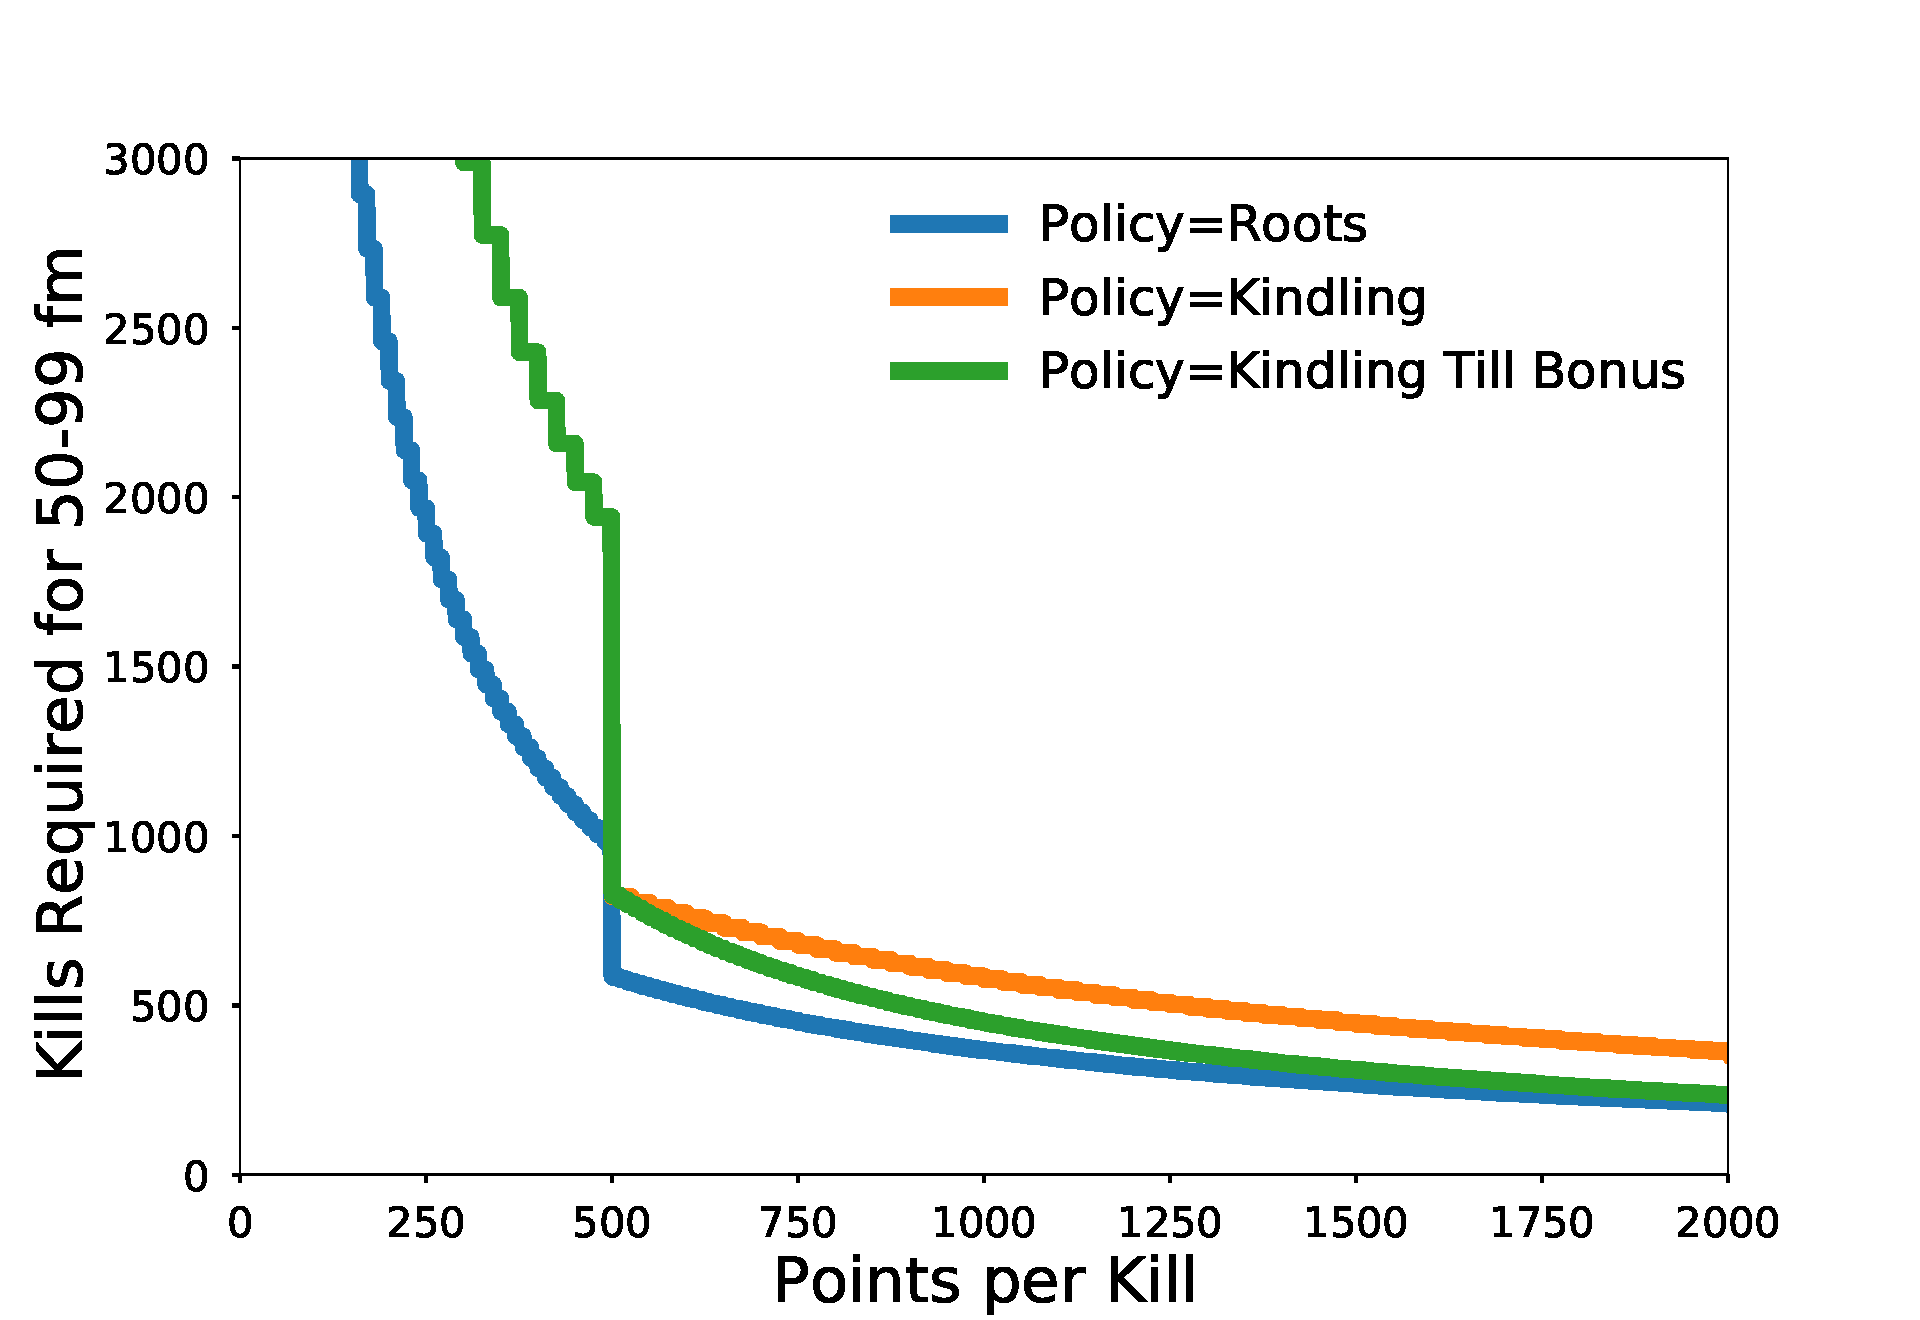
\includegraphics[width=0.9\linewidth]{policies.pdf}
		    \vspace{5mm}
		\end{subfigure}%
		\begin{subfigure}{\rcol\linewidth}
			% \textsize
			\vspace{10mm}
		    The experience gained from an action depends on the previous actions since the player may level up during a fight. After each fight, we also add in the bonus experience. So, the experience gained can be modeled as a set of two \textit{recursive} equations. The Only Burn Kindling, and Only Burn Roots policies act as upper and lower bounds for the kills required to reach a given level (for any playstyle/policy). 
		\end{subfigure}
		\vspace{5mm}
		\hrule 

		\begin{subfigure}{\lcol\linewidth}
		    \centering
		    \LARGE{\textbf{Rewards}}
		\end{subfigure}%
		\textsize
		\begin{subfigure}{\ccol\linewidth}
		    \vspace{5mm}
		    \centering
		    \begin{gather*}
			    \text{Rolls} = \begin{cases}
					\min(1 + p / 500, 28) & \text{if $p \ge 500$} \\
					0 & \text{otherwise},
				\end{cases}\\
				\text{Total Value} = \text{Kills} \times \text{Rolls} \times \text{Roll Value}
			\end{gather*}
		    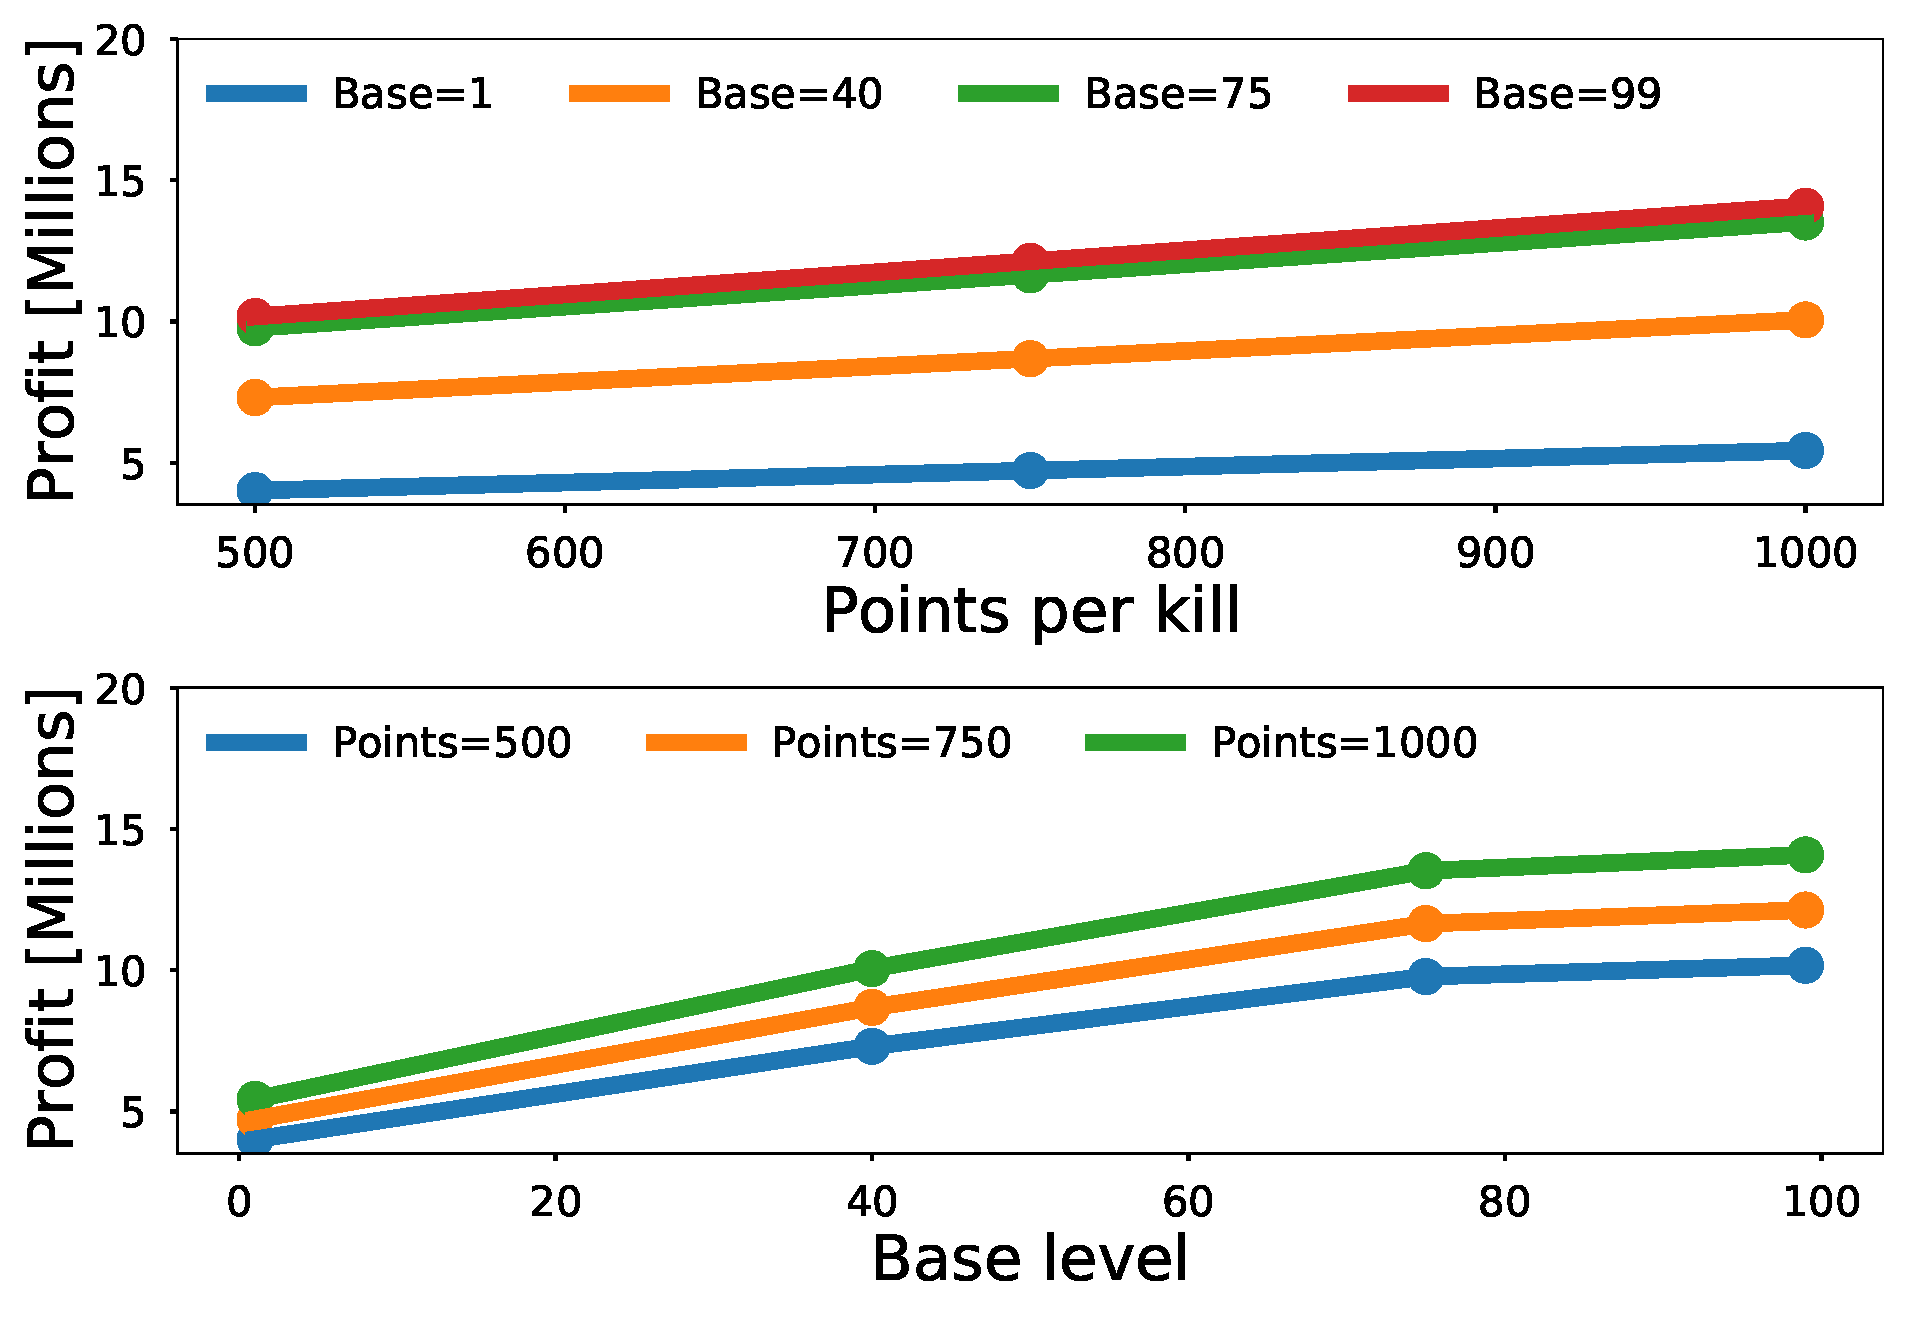
\includegraphics[width=0.9\linewidth]{profit.pdf}
		    \vspace{5mm}
		\end{subfigure}%
		\begin{subfigure}{\rcol\linewidth}
		    The value of a crate comes from some of the player's other skill levels. We can use the Wiki calculator to determine the value of a crate for a player with a base skill level. Combining this with the number of kills required gives an estimate for the total value expected over the course of 99 firemaking.
		\end{subfigure}

		\hrule 

		% \begin{subfigure}{\lcol\linewidth}
		    \vspace{5mm}
		    \centering
		    \LARGE{\textbf{Takeaways}}\\
		    \large
		% \end{subfigure}%
		% \begin{subfigure}{0.85\linewidth}
			\centering
			% \vspace{5mm}
			(Under the assumptions of this model!)
		    \begin{enumerate}
		    \centering	
		    	\item 50-99 takes a \emph{maximum} of 839 kills (70h).
		    	\item 50-99 at base 40s yields about 7-8 million gp.
		    	\item Value doesn't increase much past base 70s
		    	\item Value increases linearly as points earned increases.
		    	\item For 500 point games, 591-839 kills are required (49-70h) (for any policy!)
		    	\item For 750 point games, 455-690 kills are required (38-58h) (for any policy!)
		    \end{enumerate}
		% \end{subfigure}%
		% \vspace{5mm}\\
		\vspace{5mm}
		\hrule
		\vspace{5mm}
		\Large

		% Interested in more?\\
		% \vspace{3mm}
		Discord Chat {\HUGE \faDiscord}  \href{https://discord.gg/2B7tNUkk}{2B7tNUkk}\phantom{...}\\
		Github Project Page {\HUGE \faGithub} \href{https://github.com/Palfore/OSRSmath}{Palfore/OSRSmath}\\
		% {\HUGE \faDiscord} \url{2B7tNUkk} Interested in more? {\HUGE \faGithub} \url{Palfore/OSRSmath}\\
		
		

		% \caption[short]{A beautiful, well written caption}
	\end{figure}
\end{document}